% Requires: \usepackage{pgfplots}
%           \pgfplotsset{compat=1.18}

% Figure 1: Distribution of lde
\begin{figure}
\centering
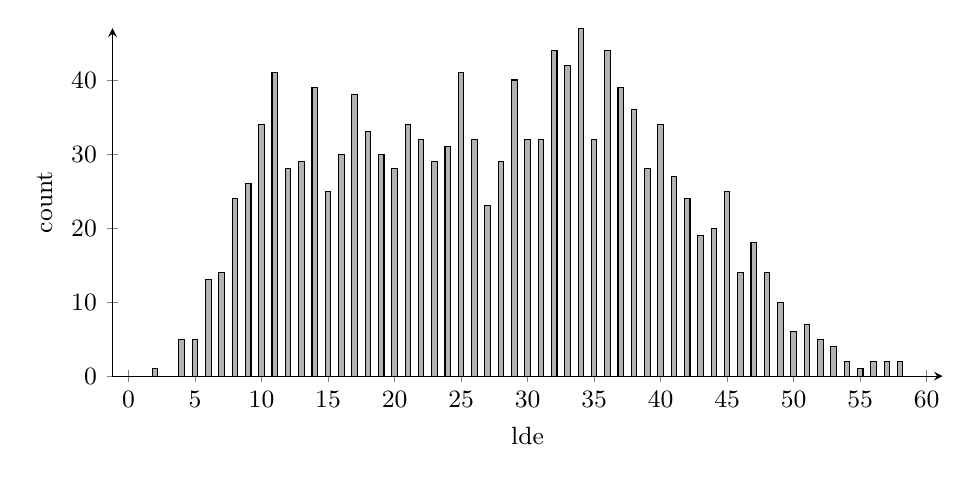
\begin{tikzpicture}
\begin{axis}[
    ybar=0pt,
    bar width=2pt,
    width=\linewidth,
    height=6cm,
    xlabel={lde},
    ylabel={count},
    ymin=0,
    xmin=0, xmax=60,
    xtick={0,5,10,15,20,25,30,35,40,45,50,55,60},
    ytick={0,10,20,30,40,50},
    tick label style={font=\small},
    label style={font=\small},
    axis lines=left,
    enlarge x limits=0.02,
]
\addplot[fill=black!30, draw=black] coordinates {
    (2,1) (4,5) (5,5) (6,13) (7,14) (8,24) (9,26) (10,34)
    (11,41) (12,28) (13,29) (14,39) (15,25) (16,30) (17,38)
    (18,33) (19,30) (20,28) (21,34) (22,32) (23,29) (24,31)
    (25,41) (26,32) (27,23) (28,29) (29,40) (30,32) (31,32)
    (32,44) (33,42) (34,47) (35,32) (36,44) (37,39) (38,36)
    (39,28) (40,34) (41,27) (42,24) (43,19) (44,20) (45,25)
    (46,14) (47,18) (48,14) (49,10) (50,6) (51,7) (52,5)
    (53,4) (54,2) (55,1) (56,2) (57,2) (58,2)
};
\end{axis}
\end{tikzpicture}
\caption{Distribution of the least denominator exponent (lde) across the
  1{,}346 test operators. The lde ranges from 2 to 58, with a mean of 27
  and a median of 28.}
\label{fig:lde-dist}
\end{figure}


% Figure 2: K-count reduction distribution (2% bins)
\begin{figure}
\centering
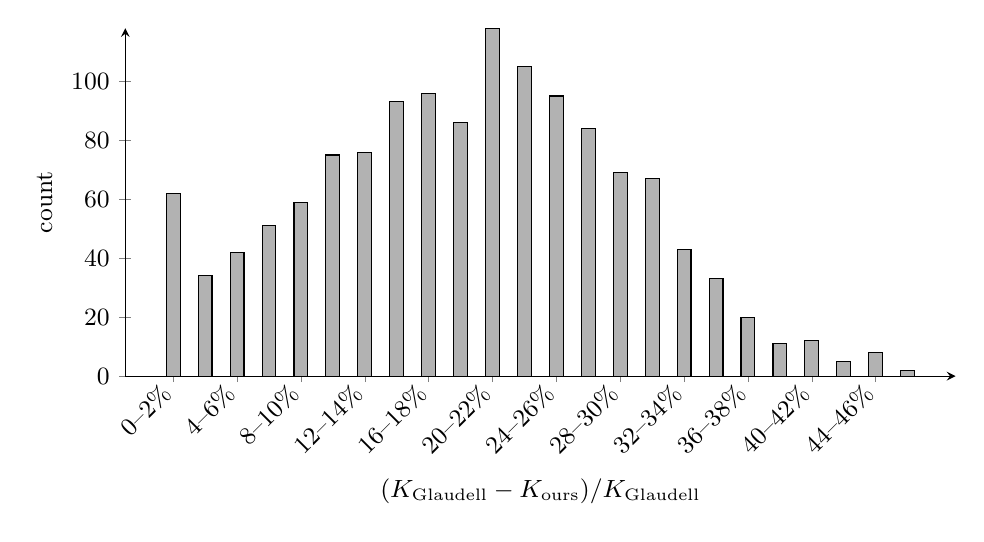
\begin{tikzpicture}
\begin{axis}[
    ybar=0pt,
    bar width=5pt,
    width=\linewidth,
    height=6cm,
    xlabel={$(K_{\mathrm{Glaudell}} - K_{\mathrm{ours}}) / K_{\mathrm{Glaudell}}$},
    ylabel={count},
    ymin=0,
    xmin=-1, xmax=49,
    xtick={1,5,9,13,17,21,25,29,33,37,41,45},
    xticklabels={0--2\%,4--6\%,8--10\%,12--14\%,16--18\%,20--22\%,24--26\%,28--30\%,32--34\%,36--38\%,40--42\%,44--46\%},
    x tick label style={font=\small, rotate=45, anchor=east},
    ytick={0,20,40,60,80,100,120},
    tick label style={font=\small},
    label style={font=\small},
    axis lines=left,
    enlarge x limits=0.02,
]
\addplot[fill=black!30, draw=black] coordinates {
    (1,62) (3,34) (5,42) (7,51) (9,59) (11,75) (13,76) (15,93)
    (17,96) (19,86) (21,118) (23,105) (25,95) (27,84) (29,69)
    (31,67) (33,43) (35,33) (37,20) (39,11) (41,12) (43,5)
    (45,8) (47,2)
};
\end{axis}
\end{tikzpicture}
\caption{Distribution of the relative $K$-count reduction
  $(K_{\mathrm{Glaudell}} - K_{\mathrm{ours}}) /
  K_{\mathrm{Glaudell}}$, binned in 2\,\% increments. Our method
  improves on Glaudell et al.'s $K$-count in 95.5\,\% of cases, with a
  mean reduction of 19.4\,\%, a median of 19.8\,\%, and a maximum of
  47.7\,\%.}
\label{fig:k-reduction-dist}
\end{figure}
